\renewcommand{\thefootnote}{\fnsymbol{footnote}}

\chapter[A Foundation for Universalisation in Games]%
        {A Foundation for Universalisation in Games\protect\footnotemark}
\label{ch:univ}

% 2) Put the actual footnote text
\footnotetext{I am indebted to Ingela Alger and François Salanié for countless discussions, comments, and invaluable guidance throughout various stages of this project. I also thank, in random order, Karine Van Der Straeten, Mostapha Diss, Alberto Grillo, Pau Juan Bartroli, Matteo Broso, Annalisa Costella, Philippe De Donder, Giacomo Rubbini, Peter Hammond, Franz Dietrich, two anonymous referees and participants at various workshops and conferences for helpful feedback. I acknowledge funding from the European Research Council (ERC) under the European Union's Horizon 2020 research and innovation programme (grant agreement No 789111 - ERC EvolvingEconomics).}

% 3) Reset things so later footnotes go back to 1, 2, 3, …
\setcounter{footnote}{0}
\renewcommand{\thefootnote}{\arabic{footnote}}


\begin{chapterabstract}
	I study the behaviour of individuals who have preferences for universalisation. When considering a course of action, they evaluate the consequence that would occur if everyone else acted equivalently, according to some criterion of equivalence. That is, they universalise their behaviour. I develop and axiomatise a model for individuals who value their choices in light of the consequences they induce when their action is universalised. The key behavioural prediction is that the independence axiom is satisfied only among actions that are universalised equivalently. I impose conditions to single out the most prominent models of universalisation, compare them, highlight and arguably overcome their limitations. I propose a unifying model of universalisation inspired by the equal sacrifice principle.
\end{chapterabstract}

\section{Introduction}\label{sec:introuniv}

What would I get if everyone acted as I do? An individual who acts based on the answer to this question exhibits universalisation reasoning. In group interactions, universalisation reasoning prescribes that individuals consider what would happen if everyone chooses the same action as them. Universalisation has been shown to have evolutionary foundations \citep{algerHomoMoralisPreference2013} and aligns with behaviour observed in experiments \citep{levineLogicUniversalizationGuides2020,miettinenRevealedPreferencesSequential2020,vanleeuwenEstimatingSocialPreferences2024}. Furthermore, it leads to desirable allocations under several normative criteria \citep{roemerKantianEquilibrium2010}.

Universalisation appears in the literature in various forms, with two prominent formulations being Homo Moralis preferences \citep{algerHomoMoralisPreference2013} and the Kantian equilibrium concept \citep{roemer2019cooperate}. Nevertheless, these models lack choice-theoretic foundations, complicating their unification and empirical testing. Without such foundations, extending the models beyond symmetric settings becomes challenging. It is unclear what \textquote{behaving in the same way} means in asymmetric contexts. Furthermore, the conceptual relationship between universalisation and other pro-social preferences remains unexplored. More worryingly, the models' predictions depend on the labels assigned to the primitive objects of choice, namely, actions in games. Universalisation prescribes considering what happens when everyone chooses the same action, therefore, changing the names of actions alters the predictions of these models. I show that developing choice-theoretic foundations for universalisation allows resolution of these issues.

I develop a model and introduce axioms that characterise preferences for universalisation. This characterisation enables the unification of previous models, rationalises existing empirical identification practices, and provides new testable predictions. I also introduce a new class of preferences for universalisation that are applicable to asymmetric settings. These preferences generalise the symmetric models, and their predictions are independent of the labelling of actions in games.

The main difficulty in modelling universalisation is that it is a non-consequentialist motivation. Preferences over actions do not depend on the material consequences these induce. Therefore, it is not straightforward to identify preferences for universalisation from choices over material consequences.\footnote{\cite{senBehaviourConceptPreference1973} suggested that non-consequentialism poses a challenge for revealed preference theory.} Economics is often resistant to considering non-consequentialist motivations \citep{fleurbaeyEconomicTheoriesJustice2019}. The classical models of \cite{anscombeDefinitionSubjectiveProbability1963} and \cite{savageFoundationsStatistics1972} illustrate this resistance. In these models, individuals rank mappings from uncertain states to consequences, usually referred to as \textquote{acts}. Preferences for an act inducing a sure consequence are equivalent to preferences for that consequence. It is impossible to rank acts according to a criterion that does not depend on their induced consequences without trivializing such a notion, for example, by including the chosen act in the description of consequences. Thus, the question is whether universalisation, as a form of non-consequentialism, can be reconciled with the consequentialist approach of choice theory without resorting to ad hoc solutions.

I show that it is fruitful to study non-consequentialist decision criteria by taking a ranking over actions in a game, not consequences, as the primitive. An example in Section \ref{sec:exampleuniv} illustrates that behaviour consistent with preferences for universalisation in a game cannot be rationalised by a preference ranking over material consequences. This motivates the use of \cite{luce1957games}'s model, where the object of choice is an element of an action set. In a two-player game, an action induces an act, a mapping between the opponent's action and a consequence of the game. The novelty is that preferences over actions are not equivalent to preferences over the induced acts. In particular, the individual cares about the consequence that would obtain if his action is universalised. For instance, in a symmetric game, the individual considers what would happen if his opponent chooses the same action as he does. To capture more general criteria for universalisation, I introduce a universalisation function that maps an individual's action to an opponent's action, given a reference profile of actions. As an example, in Multiplicative Kantian Equilibrium \citep{roemer2019cooperate}, individual actions that deviate from the reference profile by a specific proportion are universalised to opponent's action that deviates by the same proportion.

The main result, Theorem \ref{thm:sep}, provides a representation of preferences over mixed actions. The representation is a convex combination of two components. The first is the usual subjective expected utility. The second is the expected utility over the distribution of consequences obtained if the action is universalised. Therefore, preferences are a generalisation of subjective expected utility. The theorem allows to identify preferences over sure consequences up to the usual affine transformations and beliefs uniquely. The key deviation from expected utility is a violation of the independence axiom. In particular, independence holds only among actions that are universalised equivalently. Such violation of independence also constitutes a novel behavioural prediction. A direct test of a specific model of universalisation requires observing a violation of independence among actions that are universalised equivalently.

Because the theorem is silent on the shape of preferences over sure consequences, it reveals that universalisation and pro-social preferences are distinct assumptions; it is possible for an individual to exhibit both, consistent with empirical evidence \citep{vanleeuwenEstimatingSocialPreferences2024}. Moreover, the theorem implies that welfare analysis for individuals with preferences for universalisation cannot use material consequences as a currency, contrary to the standard practice in Kantian Equilibrium models \citep{roemer2019cooperate}. An individual with consequentialist preferences can always be compensated with material payoff, such as money, to refrain from taking a specific action. This is not true for individuals with preferences for universalisation, as they desire to induce a specific consequence as a result of their action being universalised. Non-consequentialist individuals thus suffer when they cannot choose the action they prefer, regardless of any material compensation. I thus argue that welfare criteria for non-consequentialist preferences may encompass a form of freedom of choice.\footnote{See, for example, \citet[Ch. 10]{fleurbaey2008fairness}.}

By specifying the universalisation function, I provide a choice-theoretic foundation for Homo Moralis preferences for universalisation à la \cite{algerHomoMoralisPreference2013} and the various definitions of Kantian Equilibrium by \cite{roemer2019cooperate}, both of which constitute a generalisation of the model by \cite{laffontMacroeconomicConstraintsEconomic1975}. I comment on the difference between my foundation for Kantian Equilibrium and that of \citeauthor{roemer2019cooperate}. He suggests that his model does not assume preferences that deviate from selfish material satisfaction, but rather a different \textquote{optimisation protocol}. I argue that his model's properties can be preserved by abandoning the distinction between the optimisation protocol and preferences, resulting in a more parsimonious framework in line with classical choice theory.

I develop a novel concept of universalisation inspired by the equal sacrifice principle \citep{mill1885principles,youngDistributiveJusticeTaxation1988}. Consider an individual with any given aim. Given a profile of actions in a game, the individual evaluates a deviation by considering the consequence that would occur if their opponents also deviated to induce an equivalent difference in aim satisfaction, that is, an equal sacrifice. I show that this form of universalisation is equivalent to that of Homo Moralis and Kantian Equilibrium in symmetric games. Moreover, its predictions do not depend on the labelling of actions, nor does its definition require the veil of ignorance construct used to define Homo Moralis in asymmetric contexts.

The paper is organized as follows: In Section \ref{sec:modeluniv}, I introduce the primitives of the model and the axioms. The main theorem is presented in Section \ref{sec:repuniv}. In Section \ref{sec:applicationsuniv}, I show how assumptions on the universalisation function allow me to derive various models of universalisation. Equal sacrifice universalisation is introduced in Section \ref{sec:esu}. Section \ref{sec:conclusionuniv} concludes the paper. A literature review and illustrative example follow.

\textit{Related literature.} In this paper, I study a decision problem as modelled in \cite{luce1957games}. The analysis builds on results by \cite{battigalliMixedExtensionsDecision2017}, who study \citeauthor{luce1957games} decision problems and connect them to the approach in \cite{anscombeDefinitionSubjectiveProbability1963}.

The model here is reminiscent of context-dependent preferences by \cite{gilboaDerivationExpectedUtility2003}. They study collections of individuals' preferences, one for each possible belief, over their actions and an uncertain state. As in this paper, the state is interpreted as opponents' choices. They also start from a primitive ranking over individuals' actions and obtain an expected utility representation in games. However, I here study a subjective beliefs setting, where these are derived from behaviour.

The intuition that non-consequentialist individuals do not care about an act because of its consequences has been highlighted by \cite{chenSocialPreferencesSacred2022}, who develop a choice-theoretic model to guide an experiment testing for the presence of non-consequentialist preferences. They argue that, to identify non-consequentialism from choice, individuals must face the possibility that their actions will not be implemented or observed by the experimenter. Their model has a different interpretation compared to mine. In their experiment, subjects knew that there was a chance that their action would not have been implemented, whereas here there is no such possibility.

The model in this paper allows me to distinguish universalisation from the related concept of magical thinking, studied from a choice-theoretic perspective by \cite{daleyMagicalThinkingRepresentation2017}. An individual exhibits magical thinking if he expects the probability the opponent selects a specific action to increase if he chooses that action. They provide axioms on behaviour in symmetric games that characterize magical thinking. I show that magical thinking and universalisation are different from a choice-theoretic perspective. An individual with preferences for universalisation does not believe he affects opponents' choice.

In this paper, I provide a choice-theoretic foundation for various models of universalisation. The two main alternatives are Homo Moralis preferences by \cite{algerHomoMoralisPreference2013,alger2016evolution,algerEvolutionPreferencesStructured2020} and Kantian Equilibrium by \cite{roemerKantianEquilibrium2010,roemerKantianOptimizationMicrofoundation2015,roemer2019cooperate}. In two-player games, Homo Moralis maximises a convex combination of his payoff and the payoff he would obtain if his opponent behaved as he does. The authors show that, among the set of continuous preferences, Homo Moralis is the only one that is  evolutionary stable for all the game protocols their model covers, when interactions take place under incomplete information, and there is assortativity in the process. The result is generalised to multiplayer games and structured populations by \cite{alger2016evolution} and \cite{algerEvolutionPreferencesStructured2020}. \cite{roemer2019cooperate} introduces a new solution concept, Kantian Equilibrium. He argues that, if individuals are Kantian rather than Nash optimisers, when considering deviating from an action profile they assume other players will deviate in an equivalent manner, where \textquote{equivalent} is defined in various ways. \citeauthor{algerHomoMoralisPreference2013} derive novel preferences from evolutionary analysis and \citeauthor{roemerKantianOptimizationMicrofoundation2015} changes the equilibrium concept, when compared with selfish/Nash individuals. I comment on the relation between these two models in the body of the paper.

This paper relates to studies of universalisation and other non-consequentialist motivations in various settings. Some of these study moral attitudes or their relation with pro-social preferences, as \cite{dewatripontMoralityMarkets2024}, \cite{ellingsenModelSocialDuties2024}, \cite{fleurbaey2023moralmotives} and \cite{laslierUniversalizationAltruism2022}. Others are applications in economic environments, including bargaining \citep{dizarlarKantianEquilibriaClass2023,juan-bartroliMoralPreferencesBargaining2024}, contract theory \citep{sarkisianTeamIncentivesMoral2017,sarkisianOptimalIncentivesSchemes2021,sarkisianScreeningTeamsMoral2021}, public goods \citep{brekkeEconomicModelMoral2003a}, social norms \citep{juan-bartroliInjunctiveNormsTheory2024}, taxation \citep{RePEc:ces:ceswps:_9867}, vaccination \citep{dedonderNashKantGametheoretic2025} and voting \citep{algerHomoMoralisGoes2022,dierksDoesUniversalizationEthics2024,grilloEthicalVotingHeterogenous2022}. Finally, there is interest in choice-theoretic models of individual moral attitudes. For example, \cite{ponthiereEpictetusianRationality2024}, \cite{ponthiere2024stoicism} and \cite{shiEndogenousSocialMinimum2024} study, respectively, Epictetianism, Stoicism and preference for a social minimum consumption level.

\subsection{Illustrative Example}\label{sec:exampleuniv}

I briefly illustrate the contribution of this paper through an example. I show that preferences for universalisation cannot be rationalised by a preference ranking over material consequences, and that predictions of previous models depends on the labeling. I then discuss the solution I propose and how it relates to the existing literature.

Two individuals play the following game. They can go left \( ( \ell ) \), middle \( ( m ) \) or right \( ( r ) \). The numbers in the table are monetary rewards.

\begin{table}[H]
	\begin{center}
		\begin{tabular}{c | c c c}
			\(\mu^{\prime}\) &                     & \(\nicefrac{1}{2}\) & \(\nicefrac{1}{2}\) \\
			\(\mu\)          & \(\nicefrac{1}{2}\) & \(\nicefrac{1}{2}\) &                     \\
			                 & \(\ell\)            & \(m\)               & \(r\)               \\
			\hline
			\(\ell\)         & \(1,1\)             & \(0,0\)             & \(0,0\)             \\
			\(m\)            & \(0,0\)             & \(0,0\)             & \(1,1\)             \\
			\(r\)            & \(0,0\)             & \(1,1\)             & \(0,0\)
		\end{tabular}
	\end{center}
	\caption{Preference reversal.}
	\label{tab:reversal}
\end{table}

Assume the row player has beliefs \(\mu\) in Table \ref{tab:reversal} and thus conjectures his opponent will play \(\ell\) or \(m\), each with probability \(\frac{1}{2}\). By choosing a mixed action, the row player can induce any distribution over consequences that mixes between \((0,0)\) for sure and \((1,1)\) or \((0,0)\) with equal probability. If the row player has preferences for universalisation, he will choose \(\ell\), since it is the action that, if implemented by everyone in this game, maximises his monetary payoff. From a revealed preference perspective, it is inferred that he prefers the lottery \(\frac{1}{2} (1,1 ) + \frac{1}{2} (0,0 )\) to the sure consequence \((0,0 )\). Now, consider a second scenario where the same individual has beliefs \(\mu^{\prime}\) in Table \ref{tab:reversal}, according to which his opponent plays \(m\) or \(r\) with probability \(\frac{1}{2}\). The feasible set of lotteries over consequences is the same as before. Actions \(m\) and \(r\) induce the midpoint between \((0,0 )\) and \((1,1 )\) whereas \(\ell\) induces the sure consequence \((0,0)\). The row player still chooses \(\ell\), as it is again the action that maximises his payoff if implemented by everyone. When \((0,0)\) was available, he revealed to prefer \(\frac{1}{2} (1,1 ) + \frac{1}{2} (0,0 )\). Nevertheless, he exhibits a preference reversal in the second scenario, thus violating the weak axiom of revealed preference. There is no complete and transitive preference relation on lotteries consistent with this choice pattern. This impossibility does not occur for consequentialist preferences defined on distributions of material consequences, such as selfishness, altruism, inequity aversion, or maximin. Therefore, functional forms for preferences for universalisation in the literature represent orderings over objects that are different from distributions over material consequences. This implies that preferences over material consequences should not be the relevant measure for welfare analysis of an individual exhibiting universalisation reasoning, contrary to what \cite{roemer2019cooperate} proposes.

This example also shows that the predictions of models of universalisation depend on the labelling of actions. To avoid the preference reversal, it would suffice to swap the labels of one individual's actions, changing \( m \) to \( r \) and vice versa. Indeed, \cite{roemer2019cooperate} discusses in multiple instances how to change the label of actions to define and employ universalisation. In Section \ref{sec:esu}, I present a novel definition of universalisation, relying on the general theory, that is equivalent under any redescription of actions.

\section{Model}\label{sec:modeluniv}

In this section, I introduce the primitives of the model and the axioms I consider. For any set \( Y \), I denote with \( \Delta ( Y ) \) the set of finite probability distributions over \( Y \).

\paragraph{Primitives.} I focus on two-player games, defined as follows.

\begin{definition}\label{def:game}
	A \textbf{two-player game} is a list \( G = ( \{1,2 \}, ( A_i, \succsim_i )_{i \in \{1,2 \}}, X,  \rho ) \), featuring:\footnote{The textbook by \cite{bonanno2018gametheory} discusses games whose primitives are ordinal preferences.}
	\begin{itemize}
		\item a finite set of actions \(A_i\) for each player \( i \);
		\item a common set of consequences \( X \);
		\item a consequence function \(\rho \colon A_i \times  A_{-i} \rightarrow X \);
		\item player \(i\)'s preferences over mixed actions \(\succsim_i \), for each player \( i \).
	\end{itemize}
\end{definition}

Each pair of pure actions \( (a_i, a_{-i} ) \) induces a consequences \( x = \rho_{a_i, a_{-i}} \) where \( x \in X \). Any mixed action \( \alpha_i \in \Delta ( A_i ) \) induces an \citeauthor{anscombeDefinitionSubjectiveProbability1963} act denoted with \( \rho_{\alpha_i} \colon A_{-i} \rightarrow \Delta ( X ) \) leading to consequence \( x \) under opponent's action \( a_{-i} \) with probability \( \rho_{\alpha_i,a_{-i}} ( x ) = \alpha_i ( \{ a_i \in A_i \: | \: \rho_{a_i,a_{-i}} = x \} ) \). Each pair of mixed actions \( (\alpha_i, \alpha_{-i}) \) induce a distribution over consequence, i.e., the constant act \( \rho_{\alpha_i, \alpha_{-i}} \in \Delta (X) \). I say that a mixed action \( \alpha_i \) induces a constant act if \( \rho_{\alpha_i, a_{-i}} (x) = \rho_{\alpha_i, a^{\prime}_{-i}} (x) \) for each pair \(a_{-i}, a^{\prime}_{-i} \) and \( x \). I assume there exist mixed actions that, under various opponent's actions, can induce every possible distribution of consequences. A sufficient condition for this to hold is that for each consequence \( x \) there exists an action \( a_i \) such that \( \rho_{a_i,a_{-i}} = x \) for each opponent's action \( a_{-i} \). I need such richness assumption to identify preferences, as usual in decision theory. However, in examples of games in this paper, usually only a subset of \( A_i \) of feasible actions is available.\footnote{See \citet[p. 631]{dekelEpistemicGameTheory2015} and references therein for a discussion on elicitation of preferences from bets in games.}

I now introduce a primitive instrumental to capture universalisation reasoning. The idea of universalisation is that, when individual \( i \) is evaluating mixed action \( \alpha_{i} \), he considers the distribution over consequences that would occur if his opponent plays equivalently, under some notion of equivalence. As an example, when the game is symmetric and the action set is the same for both players, he might consider the distribution of consequences induced when his opponent also plays \( \alpha_{i} \). Fix a reference mixed action profile \( ( \alpha^{*}_{i}, \alpha_{-i}^{*} ) \). A universalisation function \( T_{( \alpha^{*}_{i}, \alpha_{-i}^{*} )} \colon \Delta (A_{i} ) \rightarrow \Delta (A_{-i} ) \), maps individual \( i \)'s mixed action to an opponent's mixed action, given a reference profile. For each mixed action \( \alpha_i \), the corresponding \( -i \) universalised action is \( T_{\alpha^{*}_i, \alpha^{*}_{-i}} [\alpha_i] \).

Consider two pure actions inducing the same act. If the individual is consequentialist, he should be indifferent between these two actions, as they induce the same consequences under each opponent's action. Under consequentialism, it would be without loss of generality to study a game in which two actions inducing the same act are identified as the same action. However, preferences for universalisation are not consequentialist, they cannot be reduced to preferences over acts. Therefore, I impose a different notion of equivalence between actions.

I refer to two actions \(a_i\) and \(a_i^{\prime}\) as realisation equivalent if

\[ \left(\rho_{a_i}, \rho_{a_i,T_{\alpha^{*}_i, \alpha^{*}_{-i}} [a_i]}\right) = \left(\rho_{a_i^{\prime}}, \rho_{a_i^{\prime},T_{\alpha^{*}_i, \alpha^{*}_{-i}} [a_i^{\prime}]}\right) .\]

Namely, two actions are realisation equivalent when they induce the same act and the same distribution over consequences when they are universalised. Consider an individual who cares only about the act he induces and the constant act induced under universalisation reasoning. Then, he would be indifferent between two realisation equivalent actions. A game is \textbf{reduced} if realisation equivalent actions are the same action.

I study preferences over mixed actions \( \succsim_i \) of a generic individual \( i \). I introduce axioms on \( \succsim_i \) that characterise the following functional representation.

\begin{definition}\label{def:up}
	A ranking \( \succsim_i \) is a \textbf{Universalisation Preference} (\textit{UP}) with respect to the universalisation function \( T_{\alpha^{*}_i, \alpha^{*}_{-i}}\) if it is represented by

	\begin{equation}\label{eq:up}
		\begin{aligned}
			U_i(\alpha_i) = {} & (1-\kappa) \sum_{a_i, a_{-i}} \alpha_i(a_i) \mu_{i}(a_{-i}) u_i(\rho_{a_i, a_{-i}})                                       \\[1mm]
			{}                 & + \kappa \sum_{a_i, a_{-i}} \alpha_i(a_i) T_{\alpha^{*}_i, \alpha^{*}_{-i}}[ \alpha_i ](a_{-i}) u_i(\rho_{a_i, a_{-i}}) ,
		\end{aligned}
	\end{equation}

	for some utility function \(u_i \colon X \rightarrow \mathbb{R}\) and belief \(\mu_i \in \Delta (A_{-i} )\).
\end{definition}

A \textit{UP} is a linear combination of two components. The first component, weighted by \( 1- \kappa \), is a standard subjective expected utility. The individual computes the probability the action profile \( ( a_i, a_{-i} ) \) realises, which depends on his mixed action \( \alpha_i \) and his belief over opponent's actions \( \mu_{-i} \). Then, he evaluates the consequence \( \rho_{a_i, a_{-i}} \) obtained according to the utility \( u_i \). The second component, weighted by \( \kappa \), is the result of universalisation reasoning. Instead of evaluating the probability an opponent's action realises according to the belief \( \mu_i \), the individual considers the opponent's mixed action that results from universalising his action via the universalisation function \( T_{\alpha^{*}_i, \alpha^{*}_{-i}} \). As an example, when the game is symmetric, and then \( A_i = A_{-i} \), one can define the identity universalisation function as \( T_{\alpha^{*}_i, \alpha^{*}_{-i}} [ \alpha_i ] = \alpha_i \) for each \( \alpha_i \), regardless of the reference profile. I show in Section \ref{sec:applicationsuniv} that the identity universalisation function singles out Homo Moralis preferences from Equation \eqref{eq:up}.

\paragraph{Axioms.} I now introduce the axioms that characterise \textit{UP}. I start with standard axioms allowing me to obtain a utility representation of preferences over mixed actions.

\begin{axiom}\label{ax:wo}
	\labelname{axn:wo}{Weak order} (\textbf{Weak order}) Preferences \(\succsim_i\) are a continuous weak order.
\end{axiom}

\begin{axiom}\label{ax:nond}
	\labelname{axn:nond}{Non-triviality}
	(\textbf{Non-triviality}) There exist \( \alpha_i, \alpha^{\prime}_i \) such that \( \alpha_i \succ \alpha^{\prime}_i \).
\end{axiom}

I now proceed with axioms that characterise preferences for universalisation. First, the individual only satisfies independence among actions that are universalised equivalently. The intuition is as follows. If the individual was a consequentialist, he would satisfy independence, which would result in the standard independence condition among acts. However, the individual is also interested in the distribution of consequences induced when his action is universalised. A mixture of two actions induce a mixture in their corresponding universalised action. Therefore, when mixing, the distribution over consequences induced by the action and its universalised counterpart is not guaranteed to change linearly. Linearity is guaranteed only if the two actions are universalised equivalently.

\begin{axiom}\label{ax:uind}
	\labelname{axn:uind}{Universalisation Independence}
	(\textbf{Universalisation Independence}) If

	\[
		T_{\alpha^{*}_i, \alpha^{*}_{-i}} [ \alpha_i ] = T_{\alpha^{*}_i, \alpha^{*}_{-i}} [ \alpha^{\prime}_i ] = T_{\alpha^{*}_i, \alpha^{*}_{-i}} [ \alpha_{i}^{\prime \prime} ],
	\]

	then, for all \( \lambda \in (0,1)\),

	\[ \alpha \succsim_i \alpha^{\prime}_i \implies \lambda \alpha_i + (1- \lambda ) \alpha_{i}^{\prime \prime} \succsim_i \lambda \alpha^{\prime}_i + (1- \lambda ) \alpha_{i}^{\prime \prime} .
	\]
\end{axiom}

The next axiom states that, when two actions induce the same act, then their ranking depends on the distribution of consequences they induce when universalised. It restricts attention to preferences over actions that not only depend on the induced act, but also on the distribution of consequences induced by the universalised action.

\begin{axiom}\label{ax:ceval}
	\labelname{axn:ceval}{Universalisation evaluation}
	(\textbf{Universalisation evaluation}) If \( \rho_{\alpha_i} = \rho_{\alpha^{\prime}_{i}} \), then

	\[ \alpha_{i} \succsim_{i} \alpha^{\prime}_{i} \: \text{ if and only if } \: \rho_{\alpha_i, T_{\alpha^{*}_i, \alpha^{*}_{-i}} [ \alpha_i ]} \succsim_i \rho_{\alpha^{\prime}_i, T_{\alpha^{*}_i, \alpha^{*}_{-i}} [ \alpha^{\prime}_i ]} \: . \]
\end{axiom}

Lastly, I assume the individual satisfies independence among actions inducing constant acts. The reason is the following. A constant act induces the same distribution of consequences regardless of the opponent's action. Therefore, regardless of how the action is universalised, the opponent is not able to affect the distribution of consequences. There is therefore no reason to violate independence when considering constant acts.

\begin{axiom}\label{ax:lindep}
	\labelname{axn:lindep}{Lotteries independence} (\textbf{Lotteries independence}) If \( \alpha_i, \alpha^{\prime}_i \) and \( \alpha_{i}^{\prime \prime} \) induce constant acts, then for all \( \lambda \in (0,1) \),

	\[ \alpha \succsim_i \alpha^{\prime}_i \implies \lambda \alpha_i + ( 1- \lambda ) \alpha_{i}^{\prime \prime} \succsim_i \lambda \alpha^{\prime}_i + ( 1- \lambda ) \alpha_{i}^{\prime \prime} .\]
\end{axiom}

As an alternative, one could dispense from \usename{axn:lindep} and assume that all actions inducing constant acts are universalised equivalently. Then, \usename{axn:uind} would imply \usename{axn:lindep}. The next section studies the implication of imposing these axioms on preferences over mixed actions.

\section{Functional Representation}\label{sec:repuniv}

The main result of this paper shows that the axioms in the previous section are necessary and sufficient to characterise \textit{UP}.\footnote{All proofs are in Appendix \ref{app:proofsuniv}.}

\begin{theorem}\label{thm:sep}
	A ranking \( \succsim_i \) satisfies \usename{axn:wo}, \usename{axn:nond}, \usename{axn:uind}, \usename{axn:ceval} and \usename{axn:lindep} in a reduced game if and only if it is a \textit{UP}. Moreover, the utility function \( u_i \) is unique up to positive affine transformations and beliefs \( \mu_i \) are unique.
\end{theorem}

Theorem \ref{thm:sep} states that choices of mixed actions satisfying the axioms are consistent with the following utility function: when choosing the mixed action \( \alpha_i \), the individual evaluates the probability that each opponent's action \( a_{-i} \) realises according to his subjective belief \( \mu_i \). However, he also considers the distribution of consequences induced by his mixed action \( \alpha_i \) and the universalised action according to the universalisation function \( T_{\alpha^{*}_i, \alpha^{*}_{-i}} \). The two components are aggregated linearly.

I do not derive the form of \( u_i \), the individual may have any preferences over consequences. This fact clarifies the difference between my exercise and, as an example, that of \cite{rohdePreferenceFoundationFehr2010}. \cite{rohdePreferenceFoundationFehr2010} establishes conditions on a ranking over collective monetary rewards that characterise inequity aversion. In the language of the present paper, she studies the shape of \( u_i \). The axioms here imply nothing about such shape. The representation allows the individual, as an example, to both exhibit preferences for universalisation and, say, inequity aversion, as captured by \( u_i \). Then, in a game, the individual would choose the action that, if universalised, satisfies his inequity averse preference. Theorem \ref{thm:sep} thus clarifies that pro-social and non-consequentialist preferences are not exclusive. On the contrary, these two can coexist.

Lastly, Theorem \ref{thm:sep} allows marking the difference between universalisation and magical thinking. An individual exhibiting magical thinking believes he affects the opponent's probability to choose an action by choosing it himself. An individual with preferences for universalisation, instead, develops standard subjective beliefs about opponents' actions, and his behaviour does not affect them. Since beliefs are standard, their updating should be consistent with Bayes rule in dynamic settings. The first component of the utility function, representing preferences over the induced act, is standard, and therefore results on Bayesian updating holds.\footnote{See e.g. \cite{epsteinRecursiveMultiplepriors2003,ghirardatoRevisitingSavageConditional2002}.} In the next section, I study different forms of the universalisation function corresponding to particular preferences in the literature.

\section{Preferences for Universalisation}\label{sec:applicationsuniv}

In this section, I study conditions on the universalisation function under which \textit{UP} preferences are equivalent to various notions of universalisation in games. I start with Simple Kantian Equilibrium by \cite{roemer2019cooperate}, to later proceed with Homo Moralis by \cite{algerHomoMoralisPreference2013} and conclude with Multiplicative Kantian Equilibrium by \cite{roemer2019cooperate}. I supplement results with discussions on the interpretation of these concepts and the relation between them.

\subsection{Homo Kantiensis and Simple Kantian equilibrium}

In this section, I restrict attention to games with common action sets, where \(A_1= A_2 =A\). Simple Kantian Equilibrium is defined as follows.

\begin{definition}\label{definition:ske}
	An action profile \( ( \alpha, \alpha ) \) constitutes a \textbf{Simple Kantian Equilibrium} (\textit{SKE}) of a game with common action sets if, for all players \(i\) and actions \(\alpha^{\prime}\)

	\[
		\sum_{a_i, a_{-i}} \alpha (a_i) \alpha (a_{-i}) u_i(\rho_{a_i, a_{-i}}) \geq  \sum_{a_i, a_{-i}} \alpha^{\prime} (a_i) \alpha^{\prime} (a_{-i}) u_i(\rho_{a_i, a_{-i}}) .
	\]
\end{definition}

A symmetric mixed action profile constitutes a \textit{SKE} if it induces the best distribution over consequences over all symmetric mixed action profiles. I show that a \textit{SKE} can be interpreted as a Nash Equilibrium in a game between two players with \textit{Homo Kantiensis} preferences.

\begin{definition}\label{def:hk}
	A ranking \( \succsim_i \) is a \textbf{Homo Kantiensis} (\textit{HK}) preference if it is represented by

	\begin{equation}\label{eq:hk}
		U_i ( \alpha ) = \sum_{a_i, a_{-i}} \alpha (a_i) \alpha (a_{-i}) u_i(\rho_{a_i, a_{-i}}) ,
	\end{equation}

	for some utility function \(u_i \colon X \rightarrow \mathbb{R}\).
\end{definition}

When evaluating any mixed action \( \alpha \), a \textit{HK}, first introduced in \cite{laffontMacroeconomicConstraintsEconomic1975}, only considers the distribution over consequences induced when his opponent chooses \( \alpha \) as well. A \textit{HK} is a particular case of a \textit{UP} preference. If \( \kappa = 1 \) and \( T_{\alpha^{*}_i, \alpha^{*}_{-i}} [ \alpha ] = \alpha \) for each \( \alpha\), then Equation \eqref{eq:up} reduces to Equation \eqref{eq:hk}. In other words, a \textit{HK} satisfies the axioms in Theorem \ref{thm:sep} with respect to the identity universalisation function.

\begin{prop}\label{prop:ske}
	An action profile \( (\alpha, \alpha) \) constitutes a \textit{SKE} in a game with common action sets if and only if it constitutes a Nash Equilibrium between two \textit{HK}.
\end{prop}

Proposition \ref{prop:ske} thus establishes that \textit{SKE} is a Nash Equilibrium in a game between two players with preferences over mixed actions satisfying the axioms in Theorem \ref{thm:sep} with respect to the identity universalisation function. The result allows me to compare the foundation I offer for \textit{SKE} with that of \cite{roemer2019cooperate}. He argues that, contrary to other models in economics, he does not assume exotic preferences, but classical self-regarding attitudes.\footnote{See, among many others, \citet[p. 69]{roemer2019cooperate}.} What he varies, instead, is individuals' \textquote{optimisation protocol}, as he refers to it. He contrasts Nash optimisation with Kantian optimisation. Nash optimisation, he maintains, relies on the counterfactual \textquote{what would happen were I to change my action alone?}. Instead, Kantian optimisation induces the counterfactual \textquote{what would happen were I and all others to deviate equally?} This argument is echoed in the papers employing various declinations of Kantian Equilibrium.\footnote{See the papers in the literature review in Section \ref{sec:introuniv}.}

In the following, I argue that, although appealing, such reasoning cannot be backed up by classical choice theory. I do not take any stance on this point. It is legitimate to employ concepts that diverge from standard theory. Nevertheless, this incompatibility is particularly relevant here, as \citeauthor{roemer2019cooperate} relies on his distinction between preferences and optimisation protocol to derive welfare statements.

\citeauthor{roemer2019cooperate}'s description of the Nash counterfactual refers to the logic employed to check whether an action profile constitutes a Nash Equilibrium. Nevertheless, this is only vaguely related to the foundation of the concept.\footnote{\cite{battigalliGameTheoryAnalysis2023} offer a thorough discussion on the interpretation of Nash Equilibrium.} Outside contexts of long repeated interactions and adaptive dynamics, an action in a Nash Equilibrium profile is played by an individual holding correct conjectures about opponents' behaviour.\footnote{See \cite{perea2012epistemic} or \cite{dekelEpistemicGameTheory2015} and references therein.} However, players cannot perform the Nash counterfactual exercise, because they do not know what opponents will do, and are unable to evaluate the gain obtained from a unilateral deviation. An individual in a game selects the action that he considers the best one according to his beliefs about what his opponents will do. In turn, the definition of \textquote{best} is, in economics, his preference. In choice theory, observed behaviour is interpreted as revealing a preference for an object compared with others available, actions in this case. Optimisation is a mathematical technique employed to compute what the maximal element is given a primitive ranking over the objects of choice, it is not a feature of the individual or of an equilibrium concept. There is no empirical observation able to tell that two individuals have the same preferences but different optimisation protocols. If they choose differently in the same problem, by definition they have different preferences.

I show with Proposition \ref{prop:ske} that there is no need to rely on informal arguments regarding how individuals optimise. Behaviour consistent with \textit{SKE} can be interpreted as Nash Equilibrium behaviour in a game between two \textit{HK}. Therefore, \citeauthor{roemer2019cooperate} is correct in arguing that assuming individuals behave according to \textit{SKE} is different from saying that they are pro-social. Nevertheless, this does not mean that they optimise differently.

The critique above has implications for welfare analysis. \citeauthor{roemer2019cooperate}'s argument according to which, in \textit{SKE}, individuals have selfish preferences over material consequences but the optimisation protocol is different from Nash, generates confusion. As I showed in the motivating example, it is possible that an individual who plays according to \textit{SKE} does not have a complete and transitive preference, and hence a utility representation, over material consequences. I believe the closest reformulation of \citeauthor{roemer2019cooperate}'s point is that one can have preferences for universalisation even if the utility index in Theorem \ref{eq:up} for material consequences \( u_i \) is the same as that for consequences induced by universalised actions, as in \textit{UP} preferences in Equation \eqref{eq:up}. Nevertheless, this equivalence does not imply the individual would be indifferent between receiving a monetary amount and acting to induce it as a consequence of universalisation reasoning. Great care must be devoted to make welfare statements for non-consequentialist preferences over actions. Given that universalisation is a preference over actions, one interesting avenue is to consider that welfare should be evaluated in terms of the freedom the individual has in choosing an action he prefers.\footnote{\cite{laslierFreedomEconomics1998} offer a review of approaches on how to conceptualise freedom in economics.}

Proposition \ref{prop:ske} also offers a novel rationale for using mixed actions. Under expected utility, there is always a pure action in the set of best replies to probabilistic conjectures regarding opponents' behaviour. The Nash equilibrium mixed action of player \( i \) can be interpreted as strategic uncertainty from player \( -i \)'s perspective. Nevertheless, a \textit{HK} who plays a mixed action in a \textit{SKE} profile has no interest in being difficult to be predicted by his opponents. In his best reply set, there may be no pure actions. A rationale for employing mixed actions is therefore the adherence to a non-consequentialist attitude.

\subsection{Homo Moralis}\label{subsec:hm}

In this section, I exploit the representation in Theorem \ref{thm:sep} to derive Homo Moralis preferences as a special case of Equation \eqref{eq:up}. I again restrict attention to games with common action sets, to define Homo Moralis preferences as follows.

\begin{definition}
	A ranking \( \succsim_i \) is a \textbf{Homo Moralis} (HM) preference if it is represented by

	\begin{equation}\label{eq:hm}
		\begin{aligned}
			U_i ( \alpha ) = {} & (1-\kappa )\sum_{a_i, a_{-i}} \alpha (a_i) \mu_{i}(a_{-i}) u_i(\rho_{a_i, a_{-i}}) \\[1mm]
			{}                  & + \kappa \sum_{a_i, a_{-i}} \alpha (a_i) \alpha (a_{-i}) u_i(\rho_{a_i, a_{-i}}),
		\end{aligned}
	\end{equation}

	for some utility function \(u_i \colon X \rightarrow \mathbb{R}\) and belief \(\mu_i \in \Delta (A_{-i} )\).
\end{definition}

A Homo Moralis maximises a convex combination between subjective expected utility and expected payoff when both individuals play his action. Contrary to \textit{SKE}, \textit{HM} is a preference, not a property of action profiles. A \textit{HM} with \( \kappa=1 \) is a \textit{HK} and his preferences are represented by Equation \eqref{eq:hk}. A \textit{HM} is a \textit{UP} where the universalisation function is the identity, as in \textit{HK}. If \( T_{\alpha^{*}_i, \alpha^{*}_{-i}} [ \alpha ] = \alpha \) for each \( \alpha\), then Equation \eqref{eq:up} coincides with Equation \eqref{eq:hm}.

A \textit{HM} is not only interested in the consequence obtained when his action is universalised, but trades off consequentialist and non-consequentialist motives. Since \textit{HM} is partially strategic, he also cares about his opponent's action and thus his beliefs matter. However, contrary to magical thinking, a \textit{HM} exhibits standard beliefs that do not depend on his action. Such distinction rationalises current experimental practices relying on identifying beliefs of individuals with preferences for universalisation \citep{vanleeuwenEstimatingSocialPreferences2024}. Moreover, my analysis offers a new behavioural prediction to test for the presence of \textit{HM}, and therefore also of \textit{HK}: they both violate independence between mixed actions that are not universalised equivalently, according to the identity universalisation function.

Both \textit{SKE} and \textit{HM} are well-defined only in games with common action sets. \cite{algerHomoMoralisPreference2013} suggest a way to employ \textit{HM} preferences in asymmetric games. They propose to consider an incomplete information expansion of the basic game where players are not aware of their role, reminiscent of the veil of ignorance of \cite{harsanyiCardinalWelfareIndividualistic1955} and \cite{rawls1971theory}. Such incomplete information game is a symmetric interaction where a strategy is a map between role and action. Universalisation can then be defined as strategies are common across players. The authors refer to this preference as \textit{Ex-ante Homo Moralis}. Another definition of universalisation in asymmetric games is Multiplicative Kantian Equilibrium by \cite{roemer2019cooperate}. In the next section, I discuss Multiplicative Kantian Equilibrium, postponing observations on \textit{Ex-ante HM} to Section \ref{sec:esu}.

\subsection{Multiplicative Kantian equilibrium}\label{sec:mult}

In this section, I discuss the relationship between Multiplicative Kantian Equilibrium and \textit{UP}.\footnote{An equivalent analysis delivers similar results for Additive Kantian Equilibrium \citep{roemer2019cooperate}.} The solution concept is defined in games where the action space has a linear structure. It is employed when players can choose a number from the real line. For simplicity, I follow the recommendation in \citet[p. 42]{roemer2019cooperate} and consider the mixed extension of two-player two-actions games, though developing a generalisation of Multiplicative Kantian Equilibrium to multiple actions games is not trivial.

I remove the restriction to games with common action sets and assume players only have two pure actions available. For each \( \alpha_i \) and \( r \geq 0 \), I denote with \( r \cdot \alpha_i \) an operation that affects \( \alpha_i \) by the multiplicative factor \( r \) and \( 1 - \alpha_i \) by the complementary weight to obtain a probability distribution on pure actions, that is

\[ r \cdot \alpha_i :=\frac{r \alpha_i }{r \alpha_i +(1-\alpha_i)} \: .\]

\begin{definition}
	An action profile \( (\alpha_i, \alpha_{-i} ) \) constitutes a \textbf{Multiplicative Kantian Equilibrium} (\textit{MKE}) of a game if, for all players \( i \) and real numbers \( r \geq 0 \)

	\[
		\sum_{a_i, a_{-i}} \alpha_{i} (a_i) \alpha_{-i} (a_{-i}) u_i(\rho_{a_i, a_{-i}}) \geq \sum_{a_i, a_{-i}} r \cdot \alpha_{i} (a_i) r \cdot \alpha_{-i} (a_{-i}) u_i(\rho_{a_i, a_{-i}}).
	\]
\end{definition}

A mixed action profile constitutes a \textit{MKE} if it induces the best distribution over consequences when compared with all mixed action profiles that can be obtained by multiplying both actions by \( r \).\footnote{According to this definition, \( (0,0) \) is always a \textit{MKE} if it is available.} The notion is well defined as I am restricting attention to two actions. A multiplicative deviation is equivalent to moving weight from one action to the other.

Paralleling the analysis for \textit{SKE}, I show that \textit{MKE} can be interpreted as a Nash Equilibrium in a game between two individuals with Multiplicative Homo Kantiensis preferences, defined as follows.

\begin{definition}\label{definition:mhk}
	A ranking \( \succsim_i \) is a \textbf{Multiplicative Homo Kantiensis} (\textbf{MHK}) preference relative to the profile \( ( \alpha_{i}, \alpha_{-i} ) \) if it is represented by

	\begin{equation}\label{eq:mhk}
		U_i ( r \cdot \alpha_{i} ) = \sum_{a_i, a_{-i}} r \cdot \alpha_{i} (a_i) r \cdot \alpha_{-i} (a_{-i}) u_i(\rho_{a_i, a_{-i}}) ,
	\end{equation}

	for some utility function \(u_i \colon X \rightarrow \mathbb{R}\).
\end{definition}

The difference between \textit{MHK} and \textit{HK} is how actions are universalised, as illustrated in Figure \ref{fig:deviations}. A \textit{HK} only conceives both players choosing the same action. In two-player symmetric games with two actions, these profiles correspond to the diagonal of the square representing mixed actions. Instead, \textit{MHK} considers actions as multiplicative deviations from a specific profile. Universalised actions lie on the line connecting the origin and the reference profile, i.e., all the pairs in which the ratio between the two actions is preserved. A profile \( ( \alpha_i, \alpha_{-i} ) \) constitutes a \textit{MKE} if it is the preferred one for both players compared with any other on the line joining the origin and \( ( \alpha_i, \alpha_{-i} ) \). If \( ( \alpha_i, \alpha_{-i} ) \) lays on the \(45^{\circ}\) line, the two universalisation criteria are identical. In the next section, I discuss a novel version under which the universalisation criterion is endogenous and depends on the game at hand.

\tikzset{every picture/.style={line width=0.75pt}} %set default line width to 0.75pt

\begin{figure}[H]
	\centering
	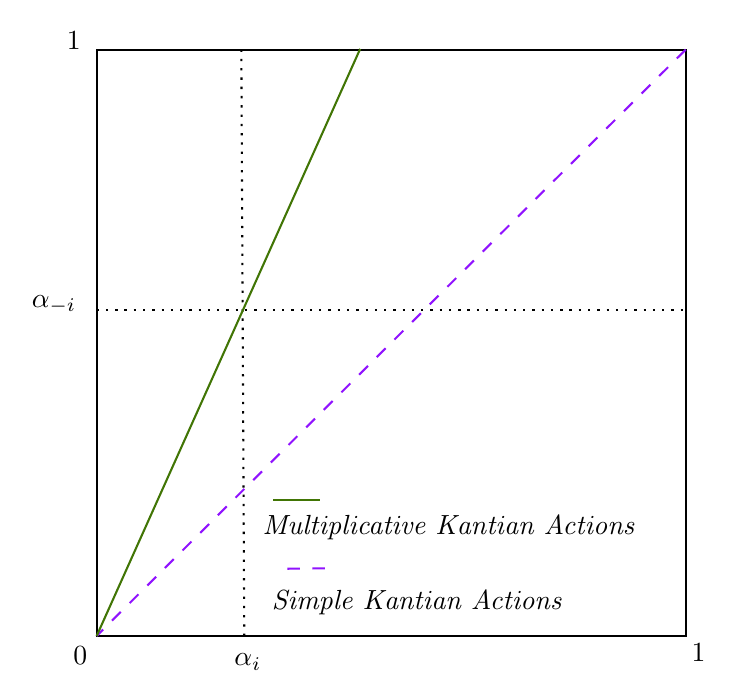
\begin{tikzpicture}[x=0.68pt,y=0.68pt,yscale=-1,xscale=1]
		%uncomment if require: \path (0,474); %set diagram left start at 0, and has height of 474

		%Shape: Rectangle [id:dp48081821398088764] 
		\draw   (141.97,35.82) -- (454.99,35.82) -- (454.99,347.39) -- (141.97,347.39) -- cycle ;
		%Straight Lines [id:da11213906072293889] 
		\draw [color={rgb, 255:red, 144; green, 19; blue, 254 }  ,draw opacity=1 ][line width=0.75]  [dash pattern={on 4.5pt off 4.5pt}]  (454.99,35.82) -- (141.97,347.39) ;
		%Straight Lines [id:da6706664054778095] 
		\draw  [dash pattern={on 0.84pt off 2.51pt}]  (141.97,174.04) -- (454.21,174.04) ;
		%Straight Lines [id:da2856973569143002] 
		\draw [line width=0.75]  [dash pattern={on 0.84pt off 2.51pt}]  (218.85,35.82) -- (220.42,347.39) ;
		%Straight Lines [id:da5420436610131965] 
		\draw [color={rgb, 255:red, 65; green, 117; blue, 5 }  ,draw opacity=1 ][line width=0.75]    (141.97,347.39) -- (282.01,35.43) ;
		%Straight Lines [id:da11662737317060468] 
		\draw [color={rgb, 255:red, 65; green, 117; blue, 5 }  ,draw opacity=1 ][line width=0.75]    (235.88,275.18) -- (260.72,275.18) ;
		%Straight Lines [id:da5716468539586732] 
		\draw [color={rgb, 255:red, 144; green, 19; blue, 254 }  ,draw opacity=1 ][line width=0.75]  [dash pattern={on 4.5pt off 4.5pt}]  (263.22,311.46) -- (239.16,311.72) ;

		% Text Node
		\draw (127.98,351.37) node [anchor=north west][inner sep=0.75pt]    {\( 0 \)};
		% Text Node
		\draw (124.54,24.71) node [anchor=north west][inner sep=0.75pt]    {\( 1 \)};
		% Text Node
		\draw (456.46,349.82) node [anchor=north west][inner sep=0.75pt]    {\( 1 \)};
		% Text Node
		\draw (105.87,164.66) node [anchor=north west][inner sep=0.75pt]    {\( \alpha _{-i} \)};
		% Text Node
		\draw (213.47,355.37) node [anchor=north west][inner sep=0.75pt]    {\( \alpha _{i} \)};
		% Text Node
		\draw (228.54,281.65) node [anchor=north west][inner sep=0.75pt]   [align=left] {\textit{Multiplicative Kantian Actions}};
		% Text Node
		\draw (233.49,321.32) node [anchor=north west][inner sep=0.75pt]   [align=left] {\textit{Simple Kantian Actions}};
	\end{tikzpicture}
	\caption{Universalised action profiles of Simple and Multiplicative Kantian Equilibria.}
	\label{fig:deviations}
\end{figure}

A \textit{MHK} is a particular case of \textit{UP} in which the actions are universalised through a multiplicative logic. If \( \kappa = 1 \) and \( T_{\alpha_i, \alpha_{-i}} [ r \cdot \alpha_i ] = r \cdot \alpha_{-i} \) for each \( r \), then Equation \eqref{eq:up} reduces to Equation \eqref{eq:mhk}.

\begin{prop}\label{prop:mke}
	An action profile \( (\alpha_i, \alpha_{-i}) \) constitutes a \textit{MKE} in a game if and only if it constitutes a Nash Equilibrium between two \textit{MHK} relative to the profile \( ( \alpha_{i}, \alpha_{-i} ) \).
\end{prop}

Proposition \ref{prop:mke} has an interpretation on the lines of its parallel result for \textit{SKE}. It establishes that \textit{MKE} is a Nash Equilibrium in a game between two players with preferences over mixed actions satisfying the axioms in Theorem \ref{thm:sep} with respect to the multiplicative universalisation function. Contrary to \textit{SKE}, \textit{MKE} can be defined when action sets are not common and allows individuals to choose heterogeneous actions, as \textit{Ex-ante HM} does. In the next section, I develop a new concept that takes a different route to define universalisation in games with general action sets.

\section{Equal Sacrifice Universalisation}\label{sec:esu}

In this section, I elaborate on the concept of universalisation and present a new notion, inspired by the equal sacrifice principle \citep{mill1885principles,youngDistributiveJusticeTaxation1988}. The model I propose has several features: its definition does not depend on the label of actions; it can be defined in asymmetric games; in symmetric games it is equivalent to \textit{HM}.

Universalisation requires the definition of two objects. First, it must be transparent what \textquote{doing the same thing} is. Second, it must be equally clear what \textquote{deviating in the same manner} means. For these two concepts to be defined, a common currency must exist for the adjective \textquote{same} to have meaning. Previous ideas employed the label of actions in games and a notion of distance between them when the action space is structured. Such an approach, I argue, is partially lacking. In most economic models, the label of actions bears no conceptual relevance and might be misleading to use it as the main ingredient of a model of universalisation. In fact, in many applications where \textit{MKE} gives intuitive results, the action labels have clear conceptual significance, as they represent effort, contribution to a public good, or use of a common resource.

I propose to use the relevant consequence of the game as a currency. In game theory, this is usually players' utility, but it can be any other index of well-being. Then \textquote{doing the same thing} and \textquote{deviating in the same manner} are interpreted as \textquote{inducing the same utility} and \textquote{inducing the same difference in utility}. The following example illustrates the idea. Consider two individuals playing the prisoners' dilemma. Numbers are Bernoulli utilities for consequences.

\begin{table}[H]
	\begin{center}
		\begin{tabular}{c | c c}
			\(\uglyfrac{\hspace*{0.1cm} 2}{1 \hspace*{0.1cm}}\) & \(a_{2}\) & \(a_{2}^{\prime}\) \\
			\hline
			\(a_{1}\)                                           & \(2,2\)   & \(0,3\)            \\
			\(a_{1}^{\prime}\)                                  & \(3,0\)   & \(1,1\)
		\end{tabular}
		\caption{Prisoners' dilemma.}
	\end{center}
\end{table}

Row player \(1\) attains his highest Bernoulli utility in \((3, 0 )\), induced by the profile \((a^{\prime}_1, a_{2} )\). I define \( \alpha_1^{s} \) as a mixed action which, compared to \( a_1^{\prime} \), given \( a_2 \), induces a reduction in expected Bernoulli utility by \( s \), i.e., \( 3 - [ 2 \alpha_1^{s} + 3 ( 1 - \alpha_1^{s} ) ] = s \). The profile leading to the highest Bernoulli utility for column player \(2\) is instead \((a_1,a_2^{\prime} )\). As for player \(2\), his mixed actions \(\alpha_2^{s}\) induces the difference \( 3 - [ 2 \alpha_2^{s} + 3 ( 1 - \alpha_2^{s} ) ] = s \). Assume that player \(1\), when picking any action \(\alpha_1^{s}\), considers a scenario where \(2\) chooses \(\alpha_2^{s}\). He envisions the consequence that would obtain if his opponent chooses the action that, if considered a unilateral deviation from \((a_1,a_2^{\prime} )\), generates the same difference in Bernoulli utility. In this game, \(\alpha_1^{s} = \alpha_2^{s} = s\) for all \(s\). Whenever they deviate from the action profile that yields their preferred material outcome, both players consider a scenario in which their opponents also deviate by choosing the same action. Therefore, the universalisation is identical to the one of \textit{HK} and \textit{HM} in this example. The actions that lead to the highest Bernoulli utility under this universalisation reasoning are \(a_1\) for \(1\) and \(a_2\) for \(2\), i.e., \( \alpha_1^{s} = \alpha_2^{s} = 1 \), the same optimal actions of \textit{HK} under proper re-labelling of actions.

Evaluating differences from the maximum attainable payoff is reminiscent of the equal sacrifice principle of \cite{mill1885principles} in the context of taxation. Hence, I dub this concept \textit{equal sacrifice universalisation} (\textit{ESU}). An individual with \textit{ESU} preferences first identifies the profile of actions inducing his preferred consequence. Second, he  evaluates each action considering the induced difference in payoff compared with the optimal action computed previously. Third, he individuates the collection of opponents' deviations that, compared with their maximal action profiles in the material dimension, lead to obtain the same absolute difference.

To ease the exposition, I here focus on equal absolute sacrifice \citep{youngDistributiveJusticeTaxation1988}. In Appendix \ref{sec:es}, I consider general equal sacrifice rules. The results and arguments in this section hold for any equal sacrifice rule. Under \usename{axn:wo}, \usename{axn:nond} and \usename{axn:lindep}, preferences over actions inducing constant acts satisfy the standard \citeauthor{anscombeDefinitionSubjectiveProbability1963} conditions. These axioms guarantee the existence of two distributions over consequence \( \overline{\gamma}, \underline{\gamma} \in \Delta (X) \) such that \( \overline{\gamma} \succsim_i \gamma \succsim_i \underline{\gamma} \) for all \( \gamma \). Then, one could define a distribution over consequences inducing sacrifice \( s \) as\footnote{The weight \( \lambda_s \) depends on the normalisation of utility. As an example, if

	\[
		\sum_{x} \overline{\gamma} (x) u_i (x) = S \: \: \text{and} \: \: \sum_{x} \underline{\gamma} (x) u_i (x) = 0,
	\]

	then \( \lambda_s = 1 - \frac{s}{S} \). In fact, by linearity \( \sum_{x} \gamma^s (x) u_i (x) = \lambda_s S \), and I would like that \( \sum_{x} \gamma^s (x) u_i (x) = S - s \), so that

	\[
		\lambda_s S = S - s \: \: \Rightarrow \: \: \lambda_s = 1 - \frac{s}{S} .
	\]}

\[ \gamma^s := \lambda_s \overline{\gamma} + (1- \lambda_s) \underline{\gamma} .\]

Then, define \( \alpha_i^{*}, \alpha_{-i}^{*} \) as any two actions such that \( \rho_{\alpha_i^{*}, \alpha_{-i}^{*}} = \overline{\gamma} \), and \( \alpha_i^s \) as any action such that \( \rho_{\alpha_i^{s}, \alpha_{-i}^{*}} = \gamma^s \). Actions \( \alpha_i^s \) leading to absolute sacrifice \(s\) by definition satisfy

\begin{equation}\label{eq:sacrifice}
	\sum_{a_{-i}} \alpha^{*}_{-i} ( a_{-i} ) \sum_{x} \rho_{\alpha^{*}_i,a_{-i}} ( x ) u_i ( x ) - \sum_{a_{-i}} \alpha^{*}_{-i} ( a_{-i} ) \sum_{x} \rho_{\alpha^{s}_i,a_{-i}} ( x ) u_i ( x ) = s .
\end{equation}

Neither \((\alpha^{*}_i, \alpha^{*}_{-i} )\) nor any \(\alpha_i^s\) are guaranteed to be unique. For the sake of the following definition, I assume they are.\footnote{Therefore, I am implicitly considering a restriction of preferences or games.}

\begin{definition}\label{def:esu}
	A ranking \( \succsim_i \) is an \textbf{Equal Sacrifice Universalisation} preference if it is represented by

	\begin{equation}\label{eq:esu}
		\begin{aligned}
			U_i ( \alpha^{s}_{i} ) = {} & (1-\kappa )\sum_{a_i, a_{-i}} \alpha^{s}_{i} (a_i) \mu_{i}(a_{-i}) u_i(\rho_{a_i, a_{-i}})         \\[1mm]
			{}                          & + \kappa \sum_{a_i, a_{-i}} \alpha^{s}_{i} (a_i) \alpha^{s}_{-i} (a_{-i}) u_i(\rho_{a_i, a_{-i}}),
		\end{aligned}
	\end{equation}

	for some utility function \(u_i \colon X \rightarrow \mathbb{R}\) and belief \(\mu_i \in \Delta (A_{-i} )\).
\end{definition}

When choosing \(\alpha^{s}_i\), the individual evaluates the scenario where his opponent deviates from the action in the profile leading to the highest Bernoulli utility to induce the same sacrifice. \textit{ESU} is a \textit{UP} in which \( T_{\alpha^{*}_i, \alpha^{*}_{-i}} [ \alpha^s_i ] = \alpha_{-i}^s \) for all \( s \), so that Equations \eqref{eq:up} and \eqref{eq:esu} coincide.

The key difference between \textit{ESU} and previous concepts is that universalisation reasoning depends on the game at hand. I illustrate this point in the battle of the sexes. Numbers are again Bernoulli utilities for consequences.

\begin{minipage}[c]{0.3\textwidth}
	\begin{table}[H]
		\begin{center}
			\begin{tabular}{c | c c}
				\(\uglyfrac{\hspace*{0.1cm} 2}{1 \hspace*{0.1cm}}\) & \(a_2\) & \(a_2^{\prime}\) \\
				\hline
				\(a_1\)                                             & \(2,1\) & \(0,0\)          \\
				\(a_1^{\prime}\)                                    & \(0,0\) & \(1,2\)
			\end{tabular}
		\end{center}
		\caption{Asymmetry.}
		\label{tab:asymmetry}
	\end{table}
\end{minipage}
\begin{minipage}[c]{0.3\textwidth}
	\begin{table}[H]
		\begin{center}
			\begin{tabular}{c | c c}
				\(\uglyfrac{\hspace*{0.1cm} 2}{1 \hspace*{0.1cm}}\) & \(a\)   & \(a^{\prime}\) \\
				\hline
				\(a\)                                               & \(2,1\) & \(0,0\)        \\
				\(a^{\prime}\)                                      & \(0,0\) & \(1,2\)
			\end{tabular}
		\end{center}
		\caption{Same Actions.}
		\label{tab:common}
	\end{table}
\end{minipage}
\begin{minipage}[c]{0.3\textwidth}
	\begin{table}[H]
		\begin{center}
			\begin{tabular}{c | c c}
				\(\uglyfrac{\hspace*{0.1cm} 2}{1 \hspace*{0.1cm}}\) & \(a\)   & \(a^{\prime}\) \\
				\hline
				\(a\)                                               & \(0,0\) & \(2,1\)        \\
				\(a^{\prime}\)                                      & \(1,2\) & \(0,0\)
			\end{tabular}
		\end{center}
		\caption{Symmetry.}
		\label{tab:symmetry}
	\end{table}
\end{minipage}

\vspace*{0.4cm}

Consider the game in Table \ref{tab:asymmetry} on the left and assume throughout that \( \kappa = 0 \) for simplicity. The table represents a standard battle of the sexes, in which player \( 1 \) would like to coordinate in the top-left corner, while player \( 2 \) would like to coordinate on the bottom-right corner. The greatest achievable payoff of both players is \(2\), in \((a_1, a_2)\) and \((a_1^{\prime}, a_2^{\prime} )\). The action \(\alpha_1^{s}\) of player \(1\) inducing a sacrifice of \(s\) solves \(2 - 2 \alpha_1^{s} = s\) and hence \(\alpha_1^{s} = \frac{2 - s}{2}\). The equivalent for player \(2\) is \(2 - (2 -  2 \alpha_2^{s}) = s\) which implies \(\alpha_2^{s} = \frac{s}{2} = 1 - \alpha_1^{s}\). The optimum for \textit{ESU} is reached at \(s= \frac{2}{3}\) with \(\alpha_1^{s} = \alpha_2^{s} = \frac{1}{2}\) which, if picked by both players, leads to a common expected payoff of \(\frac{3}{2}\).

This simple example allows me to discuss important differences between \textit{ESU} and previous concepts. First, even if we were to relabel the actions \(( a_2, a_2^{\prime})\) to \((a, a^{\prime} )\) for employing \textit{SKE}, as in the table in the middle, one would not exist anyway. The optimal action is not common, as it is \(a\) for \(1\) and \(a^{\prime}\) for \(2\). Nevertheless, I argue that the problem here is not existence. It is possible to define universalisation from an individual perspective and obtain the profile composed by subjectively optimal actions \(( a, a^{\prime} )\). This is indeed what would happen assuming both players are \textit{HK}. The issue is that it is meaningless to define \textquote{the same thing} as \textquote{the same action} in this scenario. The re-labelling of actions from Table \ref{tab:asymmetry} to \ref{tab:common} is arbitrary as any other, it is not surprising that it does not lead to intuitive results.

As a solution, \citet[p. 26]{roemer2019cooperate} suggests to relabel the game as in Table \ref{tab:symmetry} on the right, to make it symmetric. Now actions are interpreted as \textquote{do the favourite thing} and \textquote{do the least favourite thing}. The \textit{SKE} of this reformulation of the game is \(( \frac{1}{2}, \frac{1}{2} )\), i.e., the optimal actions of \textit{ESU}. Not only the optimal profile coincides, but also the set of profiles considered in the universalisation evaluation is identical. The re-labelling of actions from the first to the third table amounts to changing any mixed action \(\alpha_2^{s}\) to \(1 - \alpha_1^{s}\), which leads to \(a_2=a_1^{\prime}\) and \(a_2^{\prime}=a_1\) and switching columns. This is exactly the \textit{ESU} universalisation reasoning.

Now consider the difference between \textit{ESU} and \textit{Ex-Ante HM}. \textit{Ex-Ante HM} is defined in an incomplete information expansion of the game in which players do not know whether they will be the row player or the column player. When \(\kappa = 1\), it prescribes players to choose the strategy, in this case mapping between identity and action, that ex-ante, before identities are revealed, maximises expected utility over material consequences. The optimal strategies according to such criterion are \((a_1,a_2 )\) and \((a_1^{\prime}, a_2^{\prime} )\). Contrary to what is implemented if both players exhibit \textit{ESU}, these two profiles are Pareto-Efficient. It is already known that \textit{Ex-Ante HM} is related to utilitarian altruism \citep{laslierUniversalizationAltruism2022}. Hence, it is possible that \textit{ESU} delivers an inefficient allocation in terms of material payoff. By contrast, \textit{Ex-ante HM} is always efficient, but is indifferent to inequality.

The following result establishes that optimal actions under \textit{ESU} are always optimal actions under \textit{HK} in symmetric games and therefore the first is a generalisation of the second. The result holds for any equal sacrifice rule, not only absolute sacrifice, as shown in the proof in Appendix \ref{sec:proofs}.

\begin{prop}\label{prop:equivalent}
	Assume the game is symmetric. Then, if an action is optimal under \textit{ESU} with \( \kappa = 1 \), it is also optimal under \textit{HK}.
\end{prop}

The result may be interpreted as a conceptual robustness check. In games where \textquote{same action} has meaning, because of symmetry, \textit{ESU} delivers the intuitive universalisation evaluation of previous concepts. In asymmetric games, the universalisation evaluation depends on the equal sacrifice conception of the individual.

I conclude by addressing possible critiques to \textit{ESU}. First, it relies on interpersonal comparisons of utility, and thus is less parsimonious compared with previous concepts. I acknowledge the issue, but I argue that universalisation always relies on some form of interpersonal comparison and hence the problem is not idiosyncratic to \textit{ESU}. \textit{Ex-ante HM} also relies on the same informational requirement, as it employs the veil of ignorance construct, and thus relies on the same interpersonal comparisons of \citeauthor{harsanyiCardinalUtilityWelfare1953}'s utilitarianism. As for the various forms of Kantian Equilibrium, these rely on interpersonal comparisons of actions, as argued by \cite{sherNormativeAspectsKantian2020}, as actions need to have a cardinal interpretation common to all players. Some form of interpersonal comparisons is therefore needed also in previous conceptions.

The issue is deeper. It is not that universalisation needs some form of interpersonal comparison outside symmetric environments. It always does, but under symmetry, both concepts of \textquote{same action} and \textquote{same utility} have meaning, so comparisons of actions and utility are easy to deal with. Universalisation becomes problematic without symmetry not because of labels, but because of heterogeneity among players. The implicit suggestion of \textit{Ex-ante HM} is to solve such heterogeneity by aggregating preferences in the utilitarian fashion. MKE, instead, suggests to give actions a cardinal meaning. \textit{ESU} offers a third way.\footnote{Incidentally, \textit{ESU} is reminiscent of \cite{kalaiOtherSolutionsNashs1975} bargaining solution.}

A second issue is that \textit{ESU} might lead to corner solutions. The problem is related to the previous one. It is possible that utility indexes across players have different scales and range and this makes it hard for equal sacrifice of utility to be feasible. A partial solution is to perform a proper rescaling of utility.\footnote{Interpersonal comparisons of utility are widely discussed in social choice theory. \citet[Ch. 4]{binmoreGameTheorySocial1994a} and \citet[Ch. 7]{sen2017collective} offer critical overviews of approaches to perform this exercise.} When this is not enough, constrained versions of equal sacrifice, developed by \cite{stovallEqualSacrificeTaxation2020}, can be employed.

\section{Conclusion}\label{sec:conclusionuniv}

I developed and axiomatically characterised a model to account for non-consequentialist preferences for universalisation. The main behavioural prediction is that independence is satisfied only among actions that are universalised equivalently. I showed that the general model unifies the two most prominent models of universalisation, namely Homo Moralis and Kantian Equilibrium. Lastly, inspired by the equal sacrifice principle, I proposed a novel concept of universalisation that does not rely on the labelling of actions, is equivalent to the previous models under symmetry, and can be defined in asymmetric games. I showed how the results shed light on the conceptual underpinnings of universalisation, guide empirical work, and inform the evaluation of welfare statements. In the last paragraphs, I discuss two points regarding the methodology and implications of this paper.

I am not the first to propose changing the set of consequences to account for apparent paradoxes. \cite{baccelliCanRedescriptionsOutcomes2022}, among others, have criticised this practice, as a redescription of the problem might solve technical but not conceptual issues. They argue that it is more reasonable to capture non-material determinants of utility in the evaluation of consequences, without affecting their definition. In this paper, I adhere to this principle. I do not need to alter the set of consequences by including other features in the game. The key is to introduce a link between actions and consequences without changing these two primitives. As my introductory example shows, universalisation cannot be rationalised without assuming that the individual cares about something unrelated to the material consequences of the game. An expansion of the consequence domain is necessary. A second possibility is to include the chosen action in the description of the consequence. It would then be easy to formalise a trade-off between selecting the preferred action and maximising material payoff. This has been done in empirical work on moral preferences, notably by \cite{cappelenPluralismFairnessIdeals2007}. By contrast, my universalisation theory does not rely on assuming that an action is optimal but explains why, i.e., because it induces the preferred universalised consequence.

The final point concerns the nature of preferences for universalisation. I have denoted these as non-consequentialist, and the literature refers to them as moral. Nevertheless, I show that universalisation satisfies consequentialism under an appropriate redefinition of consequences which consider what is induced by the universalised action. What, then, is the difference between universalisation and consequentialist pro-social attitudes? John Broome argues, in \citet[p. 120]{bradleyJohnBroome2021}, that \textquote{\textit{a very specific version of consequentialism is a view I call distribution (it is often called welfarism), which is the view that the goodness of an act is determined by the goodness of the distribution of well-being that results from it}}. Universalisation is, strictly speaking, not a welfarist attitude, as the optimal action is unrelated to the distribution of well-being it induces.

\bibliographystyle{apacite}  % or another  style
\bibliography{references} % .bib file goes in ./bib/
